\documentclass[10pt]{beamer}\usepackage[]{graphicx}\usepackage[]{color}
%% maxwidth is the original width if it is less than linewidth
%% otherwise use linewidth (to make sure the graphics do not exceed the margin)
\makeatletter
\def\maxwidth{ %
  \ifdim\Gin@nat@width>\linewidth
    \linewidth
  \else
    \Gin@nat@width
  \fi
}
\makeatother

\definecolor{fgcolor}{rgb}{0.345, 0.345, 0.345}
\newcommand{\hlnum}[1]{\textcolor[rgb]{0.686,0.059,0.569}{#1}}%
\newcommand{\hlstr}[1]{\textcolor[rgb]{0.192,0.494,0.8}{#1}}%
\newcommand{\hlcom}[1]{\textcolor[rgb]{0.678,0.584,0.686}{\textit{#1}}}%
\newcommand{\hlopt}[1]{\textcolor[rgb]{0,0,0}{#1}}%
\newcommand{\hlstd}[1]{\textcolor[rgb]{0.345,0.345,0.345}{#1}}%
\newcommand{\hlkwa}[1]{\textcolor[rgb]{0.161,0.373,0.58}{\textbf{#1}}}%
\newcommand{\hlkwb}[1]{\textcolor[rgb]{0.69,0.353,0.396}{#1}}%
\newcommand{\hlkwc}[1]{\textcolor[rgb]{0.333,0.667,0.333}{#1}}%
\newcommand{\hlkwd}[1]{\textcolor[rgb]{0.737,0.353,0.396}{\textbf{#1}}}%
\let\hlipl\hlkwb

\usepackage{framed}
\makeatletter
\newenvironment{kframe}{%
 \def\at@end@of@kframe{}%
 \ifinner\ifhmode%
  \def\at@end@of@kframe{\end{minipage}}%
  \begin{minipage}{\columnwidth}%
 \fi\fi%
 \def\FrameCommand##1{\hskip\@totalleftmargin \hskip-\fboxsep
 \colorbox{shadecolor}{##1}\hskip-\fboxsep
     % There is no \\@totalrightmargin, so:
     \hskip-\linewidth \hskip-\@totalleftmargin \hskip\columnwidth}%
 \MakeFramed {\advance\hsize-\width
   \@totalleftmargin\z@ \linewidth\hsize
   \@setminipage}}%
 {\par\unskip\endMakeFramed%
 \at@end@of@kframe}
\makeatother

\definecolor{shadecolor}{rgb}{.97, .97, .97}
\definecolor{messagecolor}{rgb}{0, 0, 0}
\definecolor{warningcolor}{rgb}{1, 0, 1}
\definecolor{errorcolor}{rgb}{1, 0, 0}
\newenvironment{knitrout}{}{} % an empty environment to be redefined in TeX

\usepackage{alltt}
% \usetheme{jhsph}
\usepackage[T1]{fontenc}
\setcounter{secnumdepth}{3}
\setcounter{tocdepth}{3}
\usepackage{url}
\usepackage{graphicx}
\usepackage{multimedia}
\ifx\hypersetup\undefined
  \AtBeginDocument{%
    \hypersetup{unicode=true,pdfusetitle,
 bookmarks=true,bookmarksnumbered=false,bookmarksopen=false,
 breaklinks=false,pdfborder={0 0 0},pdfborderstyle={},backref=false,colorlinks=false}
  }
\else
  \hypersetup{unicode=true,pdfusetitle,
 bookmarks=true,bookmarksnumbered=false,bookmarksopen=false,
 breaklinks=false,pdfborder={0 0 0},pdfborderstyle={},backref=false,colorlinks=false}
\fi
\usepackage{breakurl}

\makeatletter

%%%%%%%%%%%%%%%%%%%%%%%%%%%%%% Textclass specific LaTeX commands.
 % this default might be overridden by plain title style
 \newcommand\makebeamertitle{\frame{\maketitle}}%
 % (ERT) argument for the TOC
 \AtBeginDocument{%
   \let\origtableofcontents=\tableofcontents
   \def\tableofcontents{\@ifnextchar[{\origtableofcontents}{\gobbletableofcontents}}
   \def\gobbletableofcontents#1{\origtableofcontents}
 }


\newcommand\blfootnote[1]{%
  \begingroup
  \renewcommand\thefootnote{}\footnote{#1}%
  \addtocounter{footnote}{-1}%
  \endgroup
}

\usetheme{PaloAlto}

\makeatother
\IfFileExists{upquote.sty}{\usepackage{upquote}}{}
\begin{document}

\title[]{Special Topics: Biostatistical Methods for Wearable Computing}
\subtitle[]{Analyzing ``macro" scale accelerometry data: NHANES}
\author[]{Andrew Leroux}
\makebeamertitle


% \section{Background}


% \section{Wearable and Implantable Technology}


\section{Wearable and Implantable Technology}

\begin{frame}
\frametitle{Roadmap}
\begin{itemize}
\item Last class
    \begin{itemize}
    \item Introduced accelerometry broadly
        \begin{itemize}
        \item Described what is being measured
        \item Presented some ways of visualizating the data
        \end{itemize}
    \item Provided an example of raw (sub-second level) accelerometry data
    \end{itemize}
\item Today
    \begin{itemize}
    \item Recap wearables, focusing on accelerometry
    \item Describe data and motivate dimensionality reduction (raw data to aggregated data)
    \item Describe the NHANES study
    \item Walk through some example analyses using NHANES accelerometry data
    \end{itemize}
\end{itemize}
\end{frame}



\begin{frame}
\frametitle{Wearable and Implantable Technology}
\begin{itemize}
\item Wearable and implantable devices are smart electronic devices that can be worn on the body as implants or accessories
\item Emerging technology (increasing variety of sensors and signals measured)
\item Growing popularity in health research and consumer tech
\end{itemize}
\end{frame}

\begin{frame}
\frametitle{Wearable and Implantable Technology: Statistical Methods}
\begin{itemize}
\item High dimensional time series data
    \begin{itemize}
    \item Signal processing
    \item Functional data analysis
    \item Feature extraction
    \end{itemize}
\item Methodological challenges specific to wearables
    \begin{itemize}
    \item Study protocol (device location, battery life, convenience, comfort)
    \item Wear vs non-wear (complex missing data patterns)
    \end{itemize}
\item Computational challenges
    \begin{itemize}
    \item Data storage
    \item Data analysis
    \end{itemize}
\end{itemize}
\end{frame}



\begin{frame}
\frametitle{NHANES accelerometry: Reproducing these Analyses}
\begin{itemize}
\item All analyses presented here can be replicated using the "wearables\_shortcourse\_week1.R script located at 
\url{https://github.com/andrew-leroux/wearables_special_topics_course}
\item Steps:
    \begin{itemize}
    \item Download or clone
    \item Open R project ("data\_science\_accelerometry.Rproj")
    \item Open R script "wearables\_shortcourse\_week1.R" in the "code" directory
    \item Run code
    \end{itemize}
\end{itemize}
\end{frame}


\section{Accelerometry}
\begin{frame}
\frametitle{Why Accelerometry?}
\begin{itemize}
\item Physical activity is \underline{\textbf{the}} modifiable risk factor
    \begin{itemize}
    \item Mortality 
    \item Morbidity
    \item Pain
    \item ``Aging''
    \end{itemize}
\item Objective vs. self-reported PA 
    \begin{itemize}
    \item Recall bias
    \item Subjective assessment of intensity 
    \item Questionairre format
    \item ``MET" equivalents
    \end{itemize}
\end{itemize}
\end{frame}


\subsection{Data Resolution}

\begin{frame}
\frametitle{Accelerometry: Data Reduction}
\begin{itemize}
\item Raw accelerometry data are enormous
\item A tri-axial accelerometer recording at 50hz for 7 days generates $90,720,000$ data points per subject
\item Can we reduce the data? 
    \begin{enumerate}
    \item Collapse the three channels (x,y,z) into a single time series
    \item Summarize within an epoch (1s, 5s, 1min, ...)
        \begin{itemize}
        \item ''Activity count''
        \item Activity index
        \item Vector magnitude
        \item Mean amplitude deviation
        \end{itemize}
    \end{enumerate}
\item Choices for data redution depend on study goals
\end{itemize}
\end{frame}


% 
% \begin{frame}
% \frametitle{Accelerometry: Data Reduction}
% 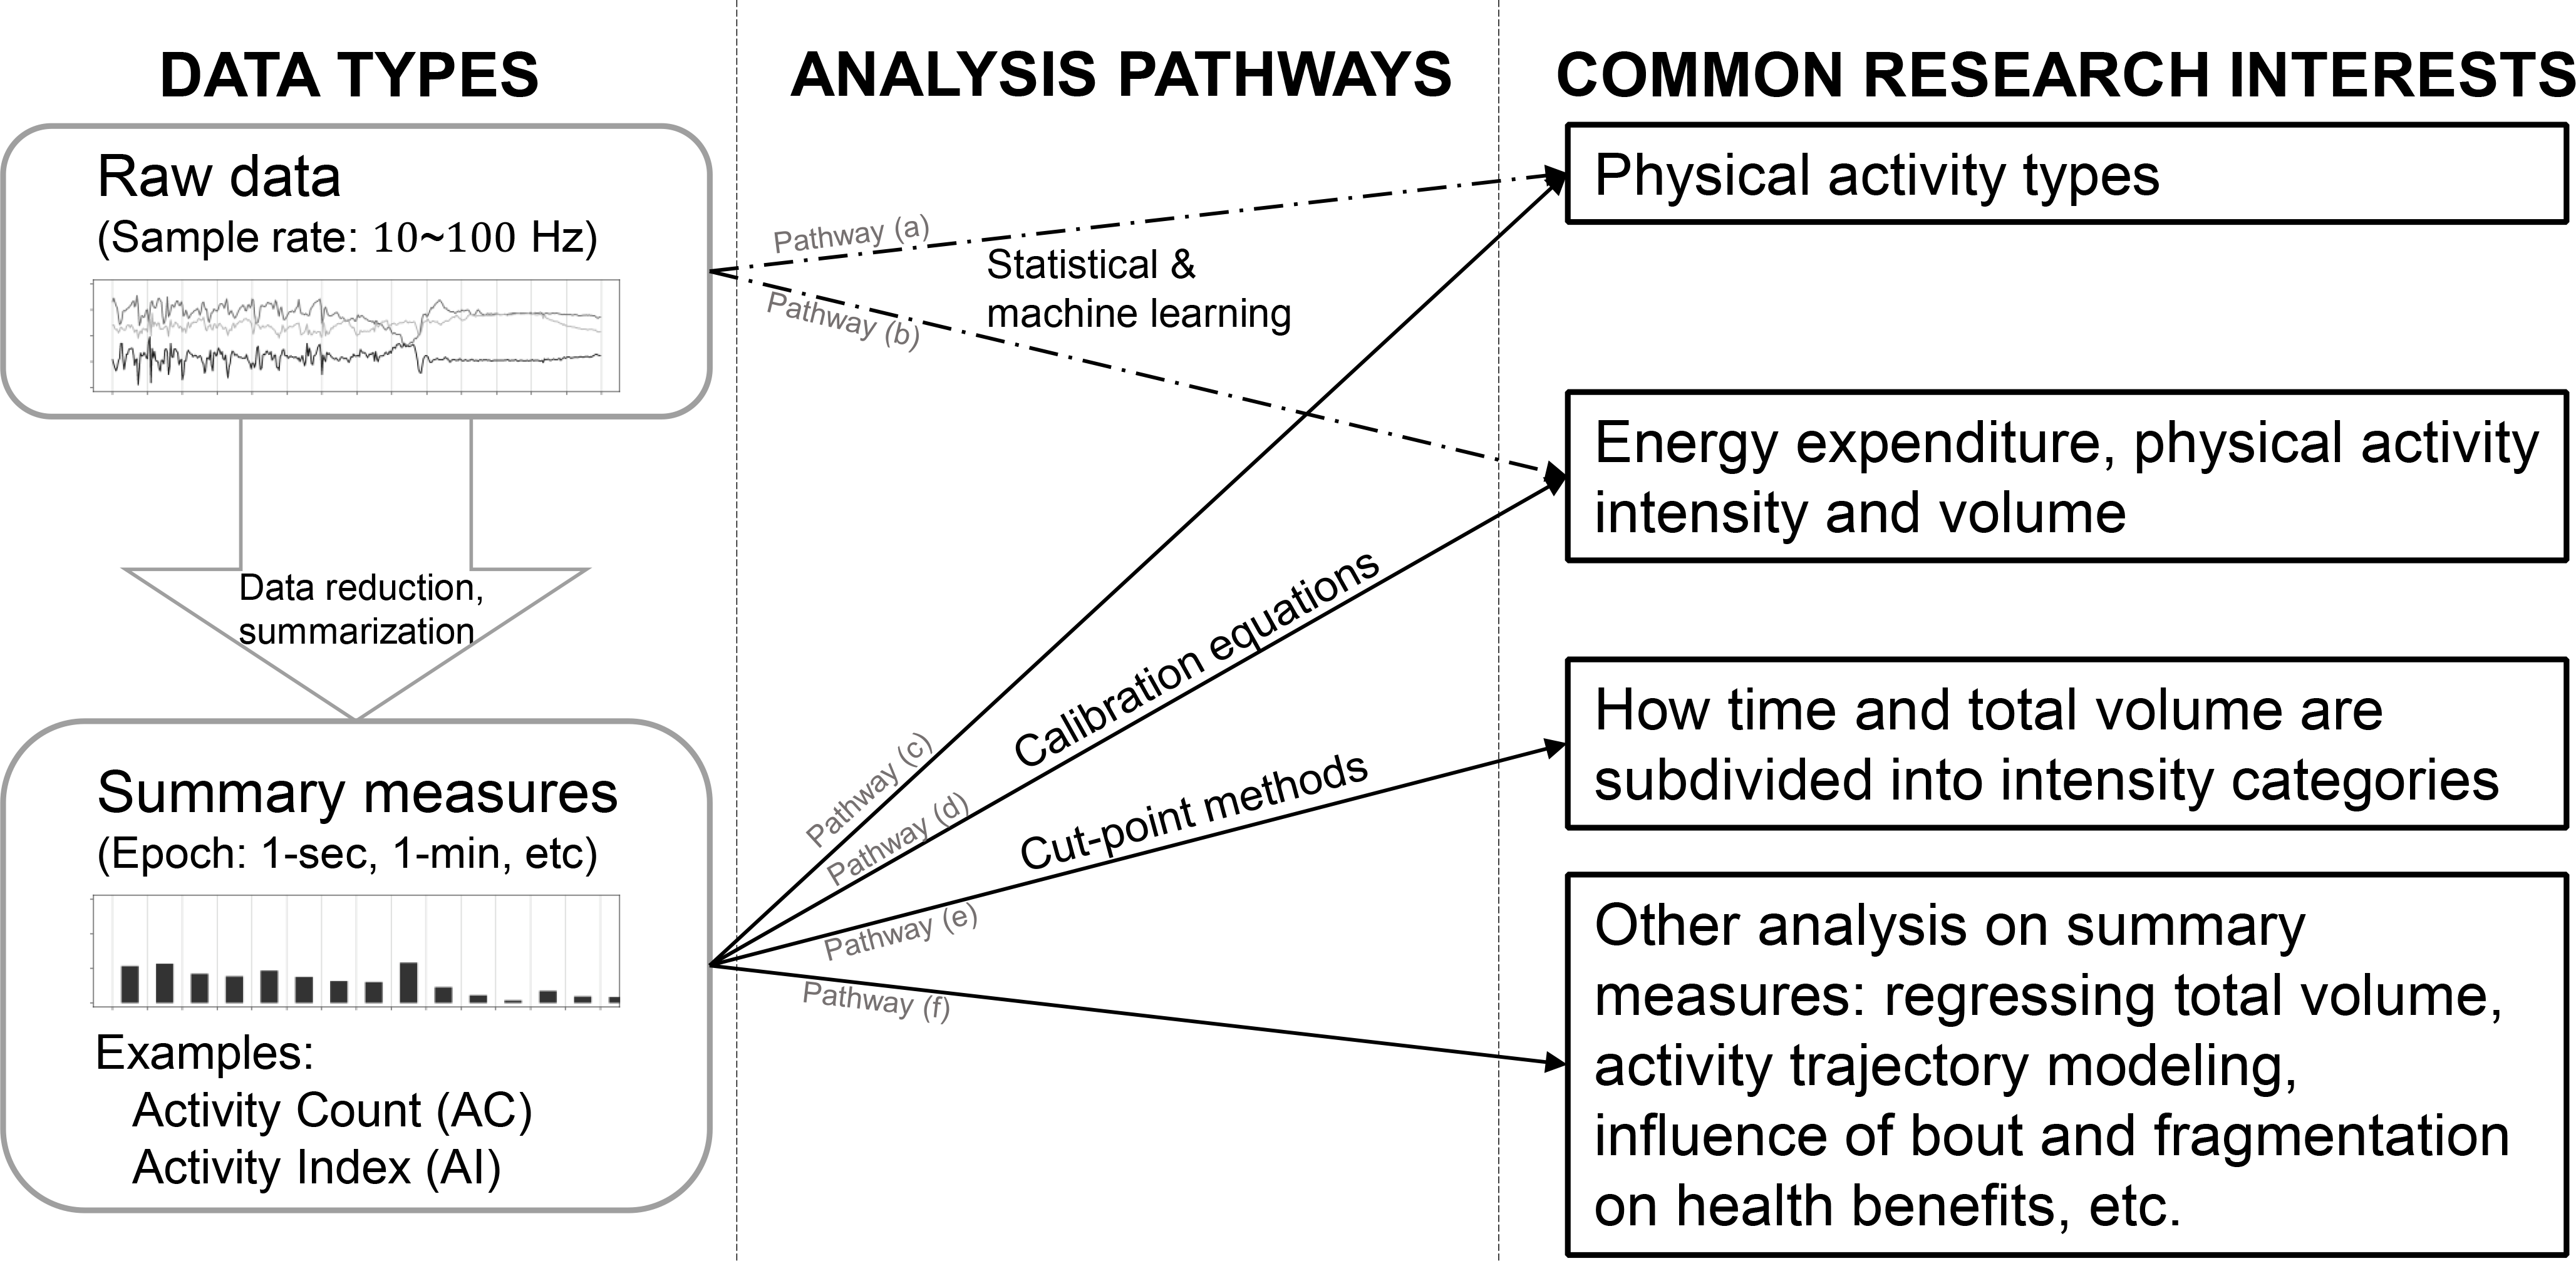
\includegraphics[width=\textwidth]{bai2016}
% \blfootnote{Bai J, Di C, Xiao L, Evenson KR, LaCroix AZ, et al. (2016) An Activity Index for Raw Accelerometry Data and Its Comparison with Other Activity Metrics. PLOS ONE 11(8): e0160644. \url{https://doi.org/10.1371/journal.pone.0160644}}
% \end{frame}

\begin{frame}
\frametitle{Micro- vs Macro-Scale Accelerometry Data}
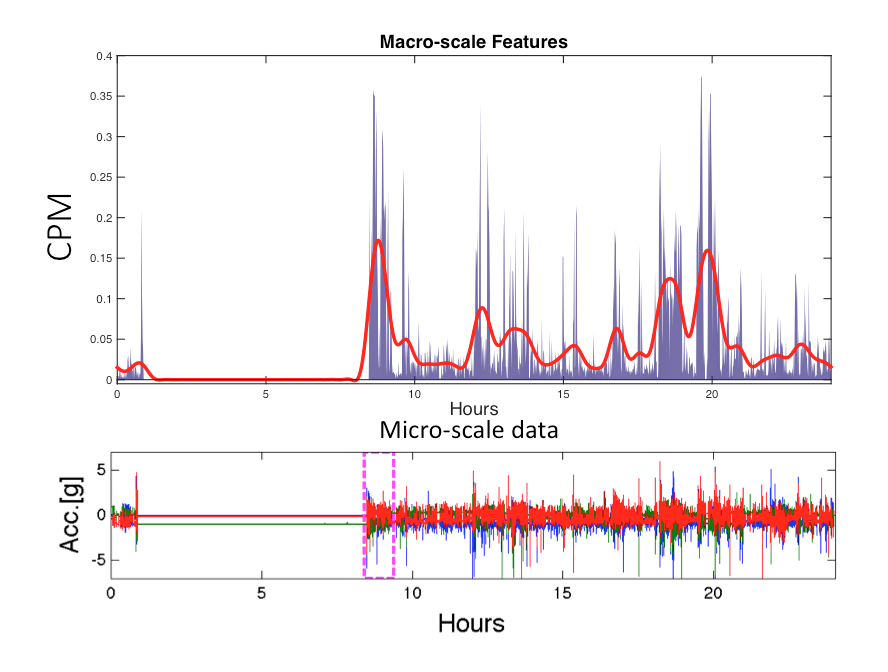
\includegraphics[width=\textwidth]{micro_vs_macro_accel_data}
\end{frame}





\section{NHANES}

\begin{frame}
\frametitle{National Health and Nutrition Examination Survey (NHANES)}
\begin{itemize}
\item Complex, multistage probability sample of the non-institutionalized US population
\item Ongoing cross-sectional study conducted in 2-year ``waves''
\item 2003-2004 and 2005-2006 waves collected accelerometry data
\item Oversamples certain groups
    \begin{itemize}
    \item African Americans, Mexican Americans
    \item Low income White Americans
    \item Adolescents (12-19 years old)
    \item Older adults (60+)
    \end{itemize}
\item All participants assigned a ``weight" indicating the number of people in the US population they ``represent''
\end{itemize}

\end{frame}


\begin{frame}
\frametitle{NHANES Sampling Procedure}
\centering
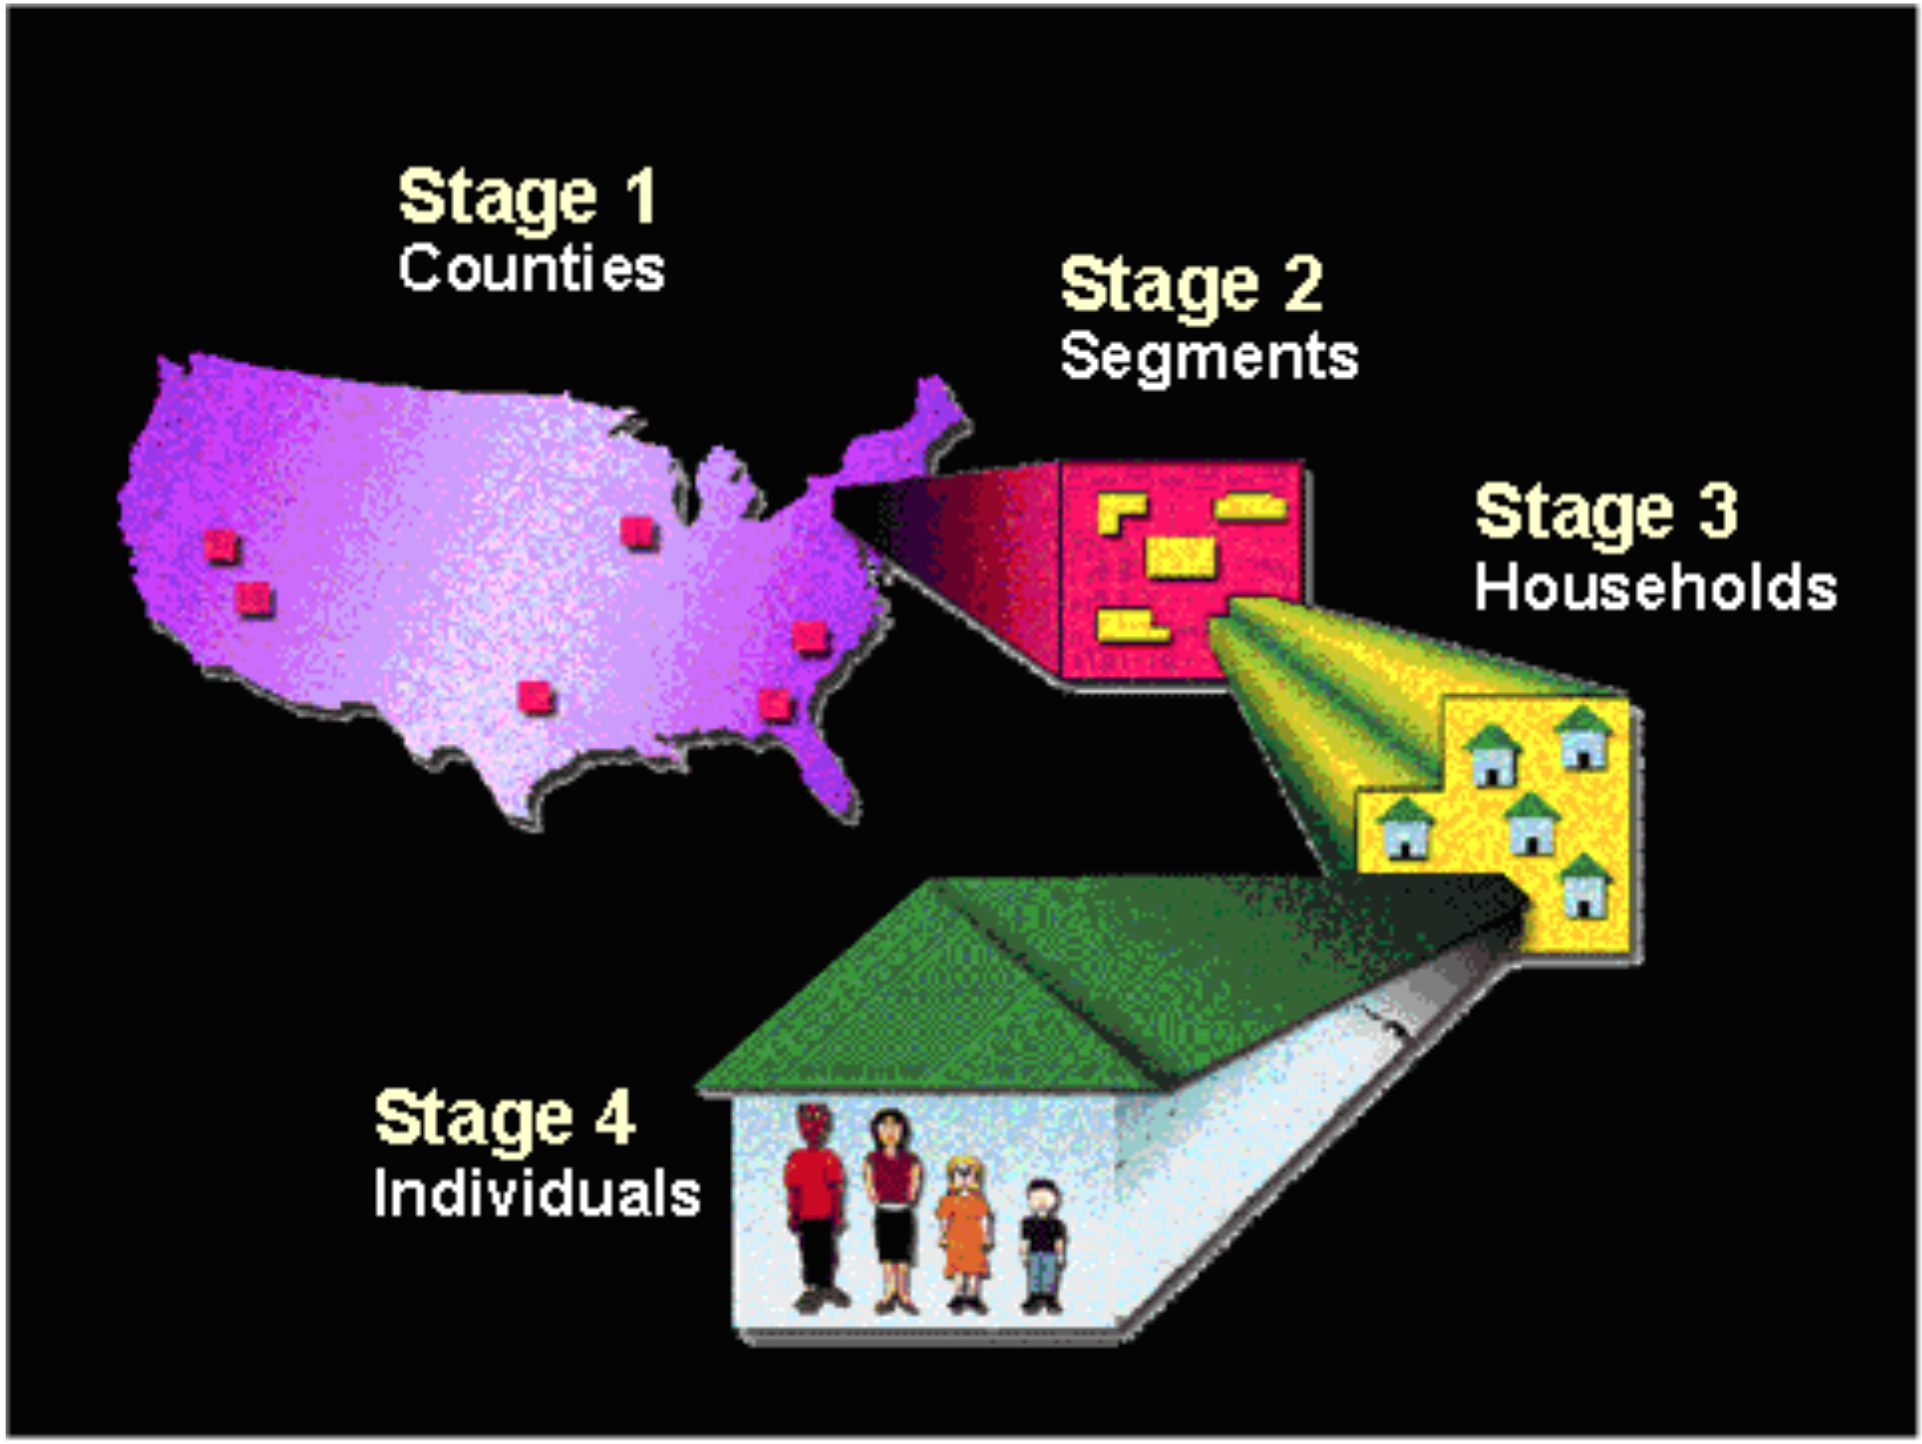
\includegraphics[width=0.8\textwidth]{NHANES_sampling}
\blfootnote{Image credit: \url{https://www.cdc.gov/nchs/tutorials/NHANES/SurveyDesign/SampleDesign/Info1.htm}}
\end{frame}



\section{An NHANES data package}

\begin{frame}
\frametitle{NHANES 2003-2006 Data}
\begin{itemize}
\item Accelerometry data
    \begin{itemize}
    \item Acceleration summarized into minute-level "activity counts"
    \item Up to 7 days of data for each participant
    \item Study protocol: remove the device at bedtime
    \end{itemize}
\item NHANES collects a lot of data on participants 
    \begin{itemize}
    \item \url{https://wwwn.cdc.gov/nchs/nhanes/ContinuousNhanes/Default.aspx?BeginYear=2003}
    \item \url{https://wwwn.cdc.gov/nchs/nhanes/ContinuousNhanes/Default.aspx?BeginYear=2005}
    \end{itemize}
\end{itemize}
\end{frame}



\begin{frame}
\frametitle{NHANES accelerometry: data structure}
\begin{itemize}
\item Accelerometry data downloadble from NHANES is in long format
\item Very large file sizes ($\approx$ 2.5 GB)
\end{itemize}
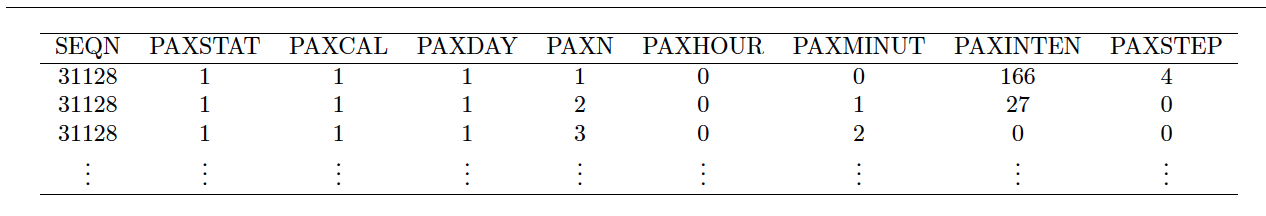
\includegraphics[width=\textwidth]{accel_data_long}
\end{frame}



\begin{frame}
\frametitle{NHANES accelerometry: proposed data strucutre}
\begin{itemize}
\item Wide format instead of long format\footnotemark ($\approx$ 60 MB)
\item 7 rows per participant, descending cronologoical order
\end{itemize}
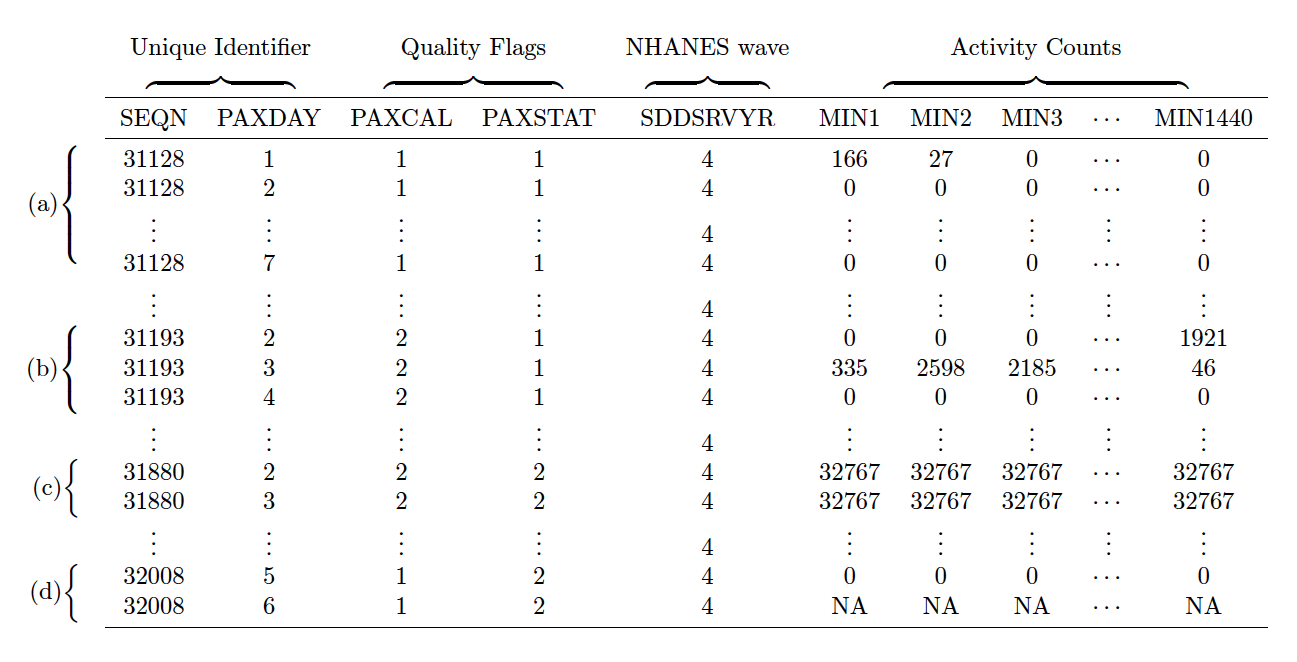
\includegraphics[width=\textwidth]{accel_data_wide}
\footnotetext{Leroux A, Di J, Smirnova E, et al. Organizing and Analyzing the Activity Data in NHANES. Statistics in Biosciences. 2019. 10.1007/s12561-018-09229-9.}
\end{frame}



\begin{frame}
\frametitle{NHANES accelerometry: {\it rnhanesdata} package}
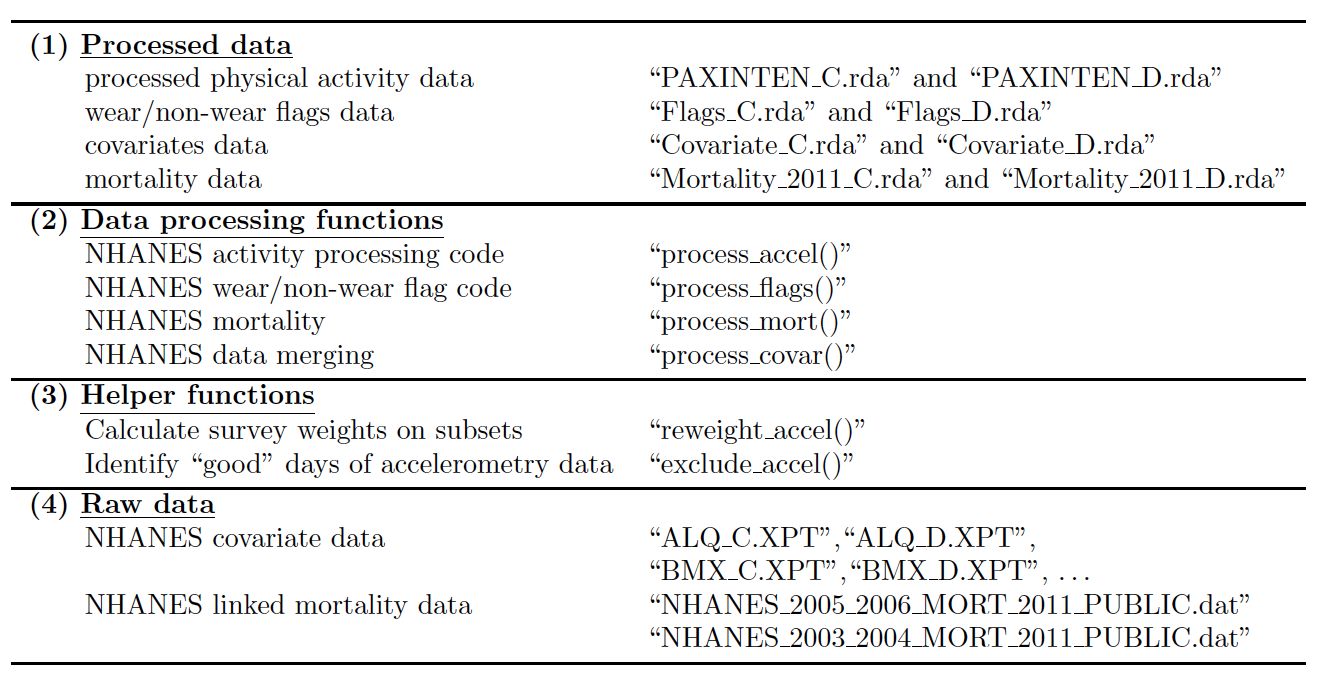
\includegraphics[width=\textwidth]{rnhanesdata}
\footnotetext{Leroux A, Di J, Smirnova E, et al. Organizing and Analyzing the Activity Data in NHANES. Statistics in Biosciences. 2019. 10.1007/s12561-018-09229-9.}
\end{frame}




\begin{frame}
\frametitle{Macro Scale Accelerometry Data: Compliant Participant}
\centering
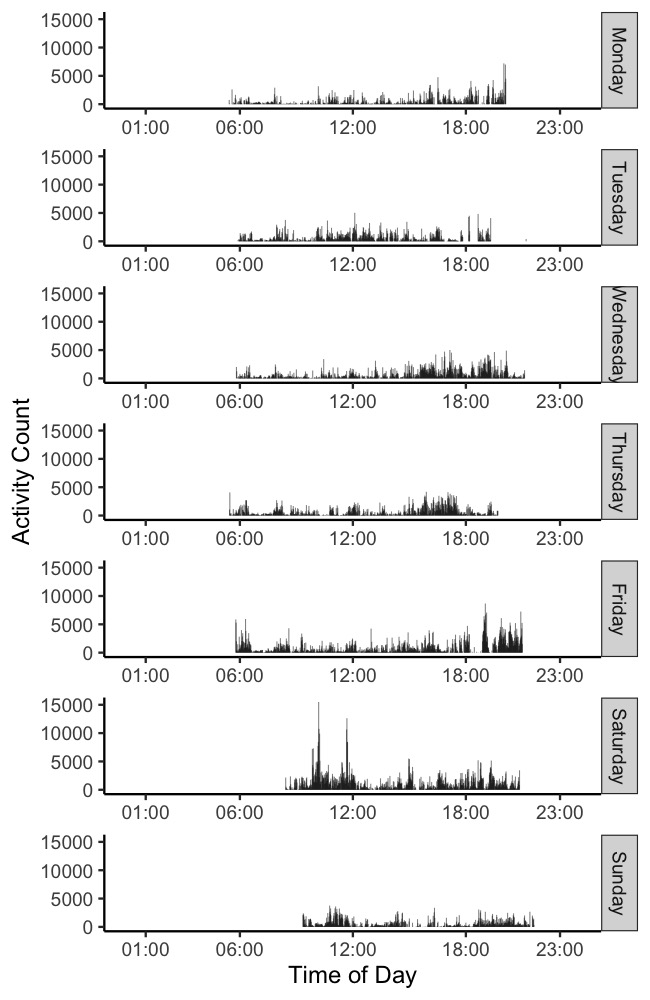
\includegraphics[height=\textheight]{profile_id1}
\end{frame}

\begin{frame}
\frametitle{Macro Scale Accelerometry Data: Compliant vs Non-Compliant Participant}
\centering
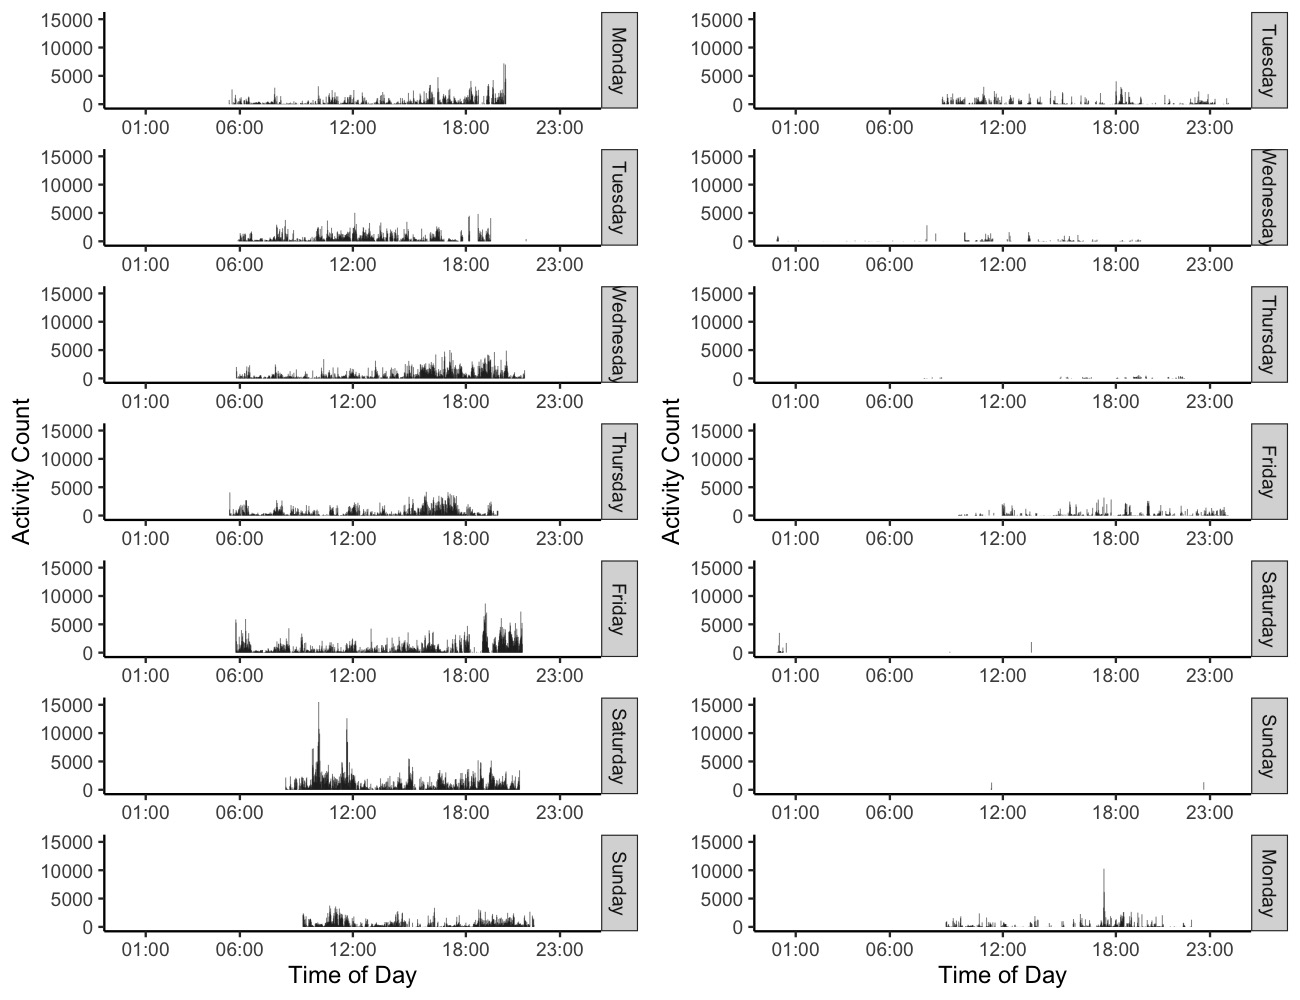
\includegraphics[height=\textheight]{profile_id1_id2}
\end{frame}


% \begin{frame}
% \frametitle{Macro Scale Accelerometry Data: Compliant vs Non-Compliant Participant}
% \centering
% 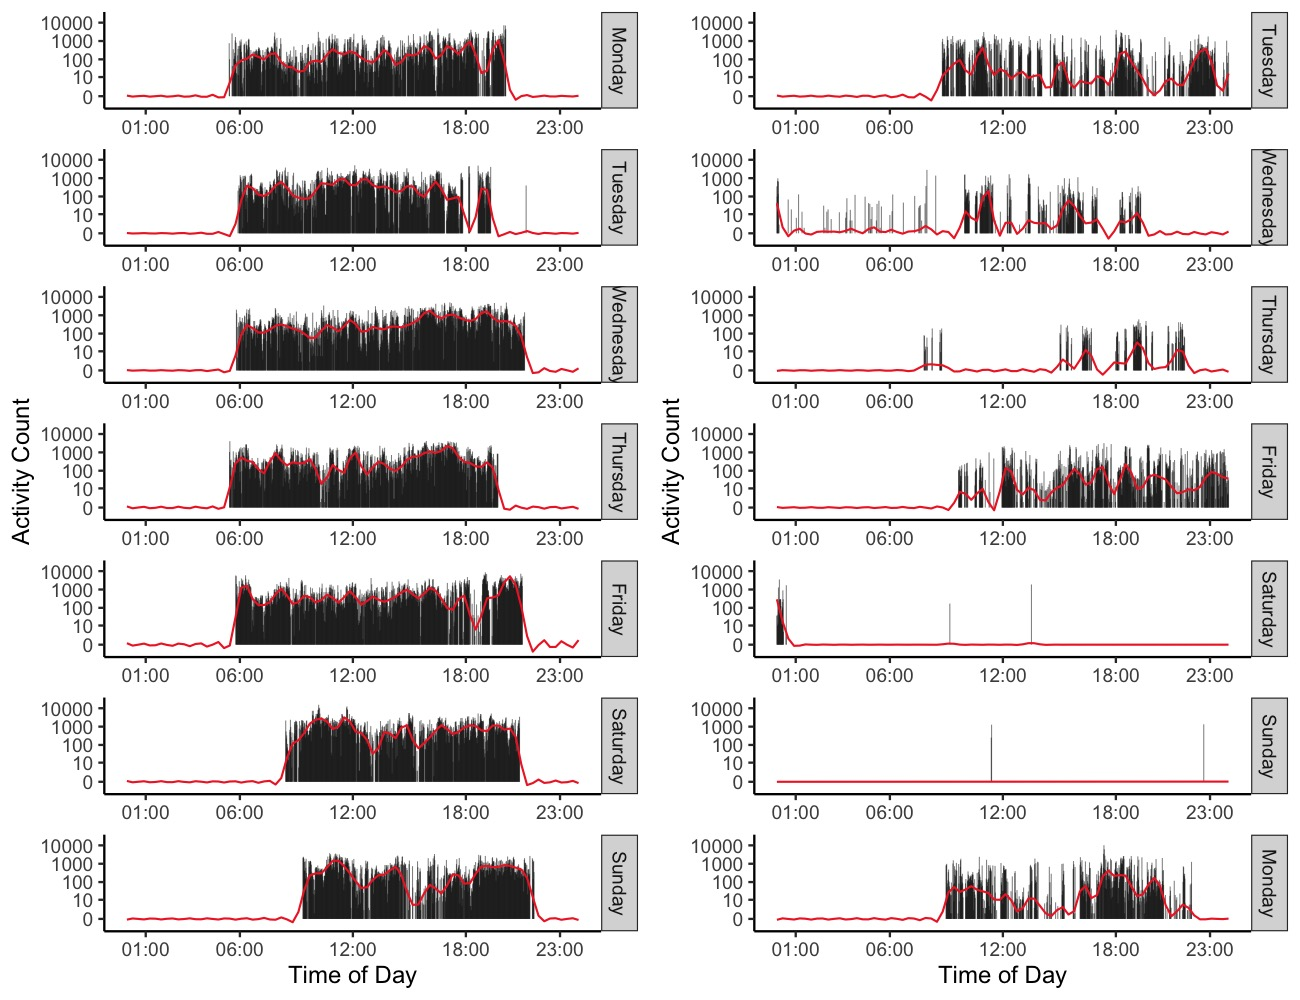
\includegraphics[height=\textheight]{profile_id1_id2_log}
% \end{frame}



\section{Analysis and Feature Extraction}






\begin{frame}
\frametitle{NHANES accelerometry: Analysis Procedure}
\begin{itemize}
\item Load and merge any relevant data by unique identifier (SEQN)
\item Apply exclusion criteria
    \begin{itemize}
    \item Data quality: 1) device calibration (PAXCAL); and 2) NHANES supplied flag (PAXSTAT)
    \item Adherence to wear-time protocol. Most studies use $\geq 10$ hours.
    \item Sufficient number of days of data. Most studies use $ \geq 3$ days of data with $\geq 10$ hours of wear.
    \item Other criteria: missing data, etc.
    \end{itemize}
\item Calculate features of interest
\item Incorporate survey design? Survey weights?
\item Regresison, machine learning, etc.
\end{itemize}
\end{frame}

\begin{frame}
\frametitle{Macro Scale Accelerometry Data: Features and Dimensionality Reduction}
\centering
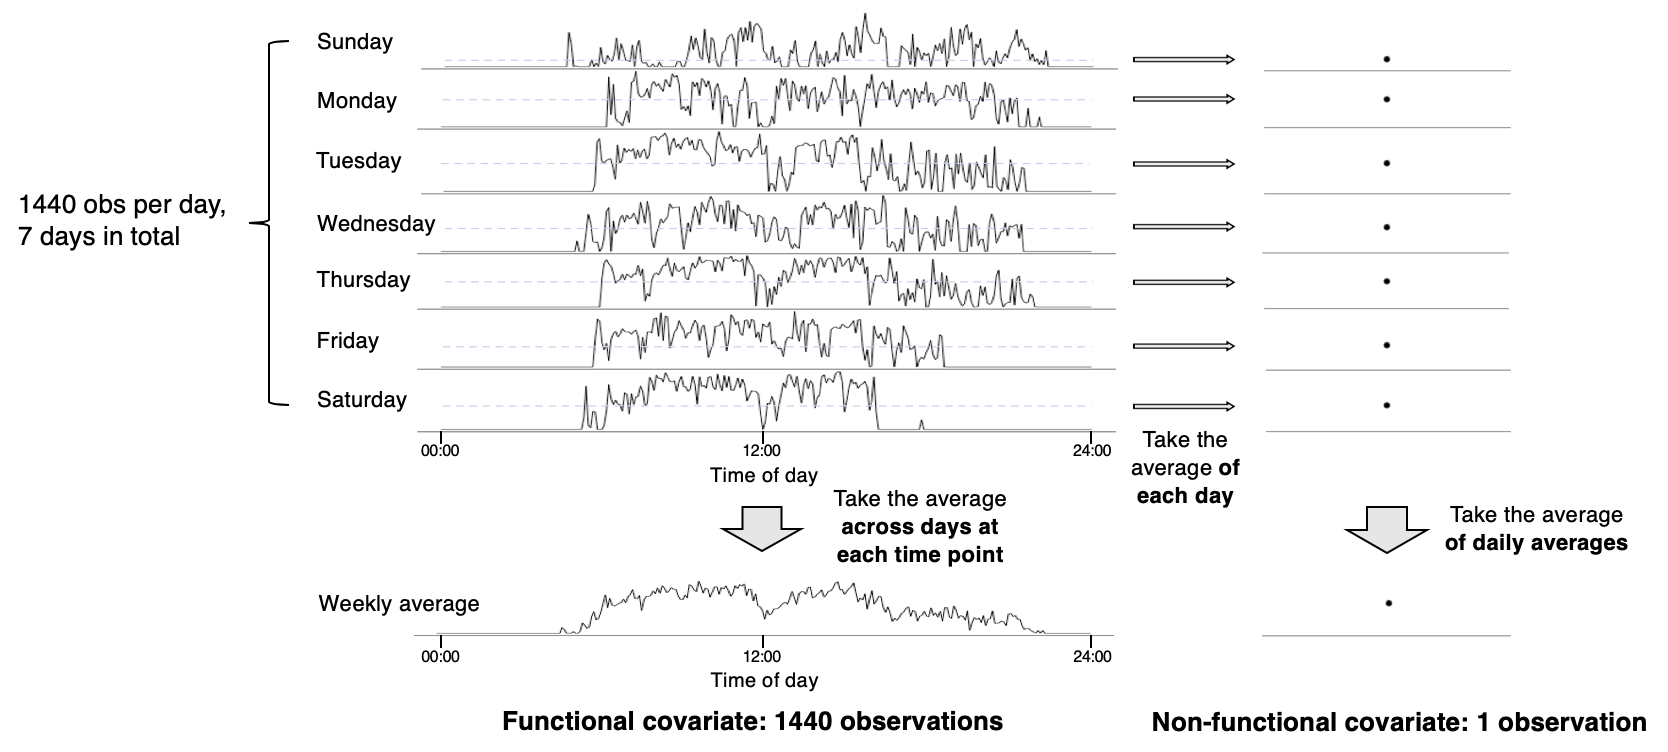
\includegraphics[width=\textwidth]{data_reduction}
\blfootnote{Image credit: Erjia Cui}
\end{frame}



\begin{frame}
\frametitle{NHANES accelerometry: Features}
\begin{itemize}
\item Analyzing activity profiles falls under ''Functional Data Analysis''
\item Current standard: calculate single summaries of the data
    \begin{itemize}
    \item Volume of activity\footnotemark
        \begin{itemize}
        \item Time spent in sedentary/light/moderate/vigorous behaviours. Require population-specific studies to determine thresholds.
        \item Average daily total activity count (TAC). A proxy for total volume of moderate/vigorous activity
        \item Average daily total log activity count (TLAC). A proxy for total volume of low/light activity
        \end{itemize}
    \item Patterns of activity
        \begin{itemize}
        \item Fragmentation measures\footnotemark
        \item Timing of physical activity (activity profiles)
        \end{itemize}
    \end{itemize}
\end{itemize}
\footnotetext{Varma VR, Dey D, Leroux A, et al. Total volume of physical activity: TAC, TLAC or TAC($\lambda$). Prev Med. 2017;106:233-235.}
\footnotetext{Di, J., Leroux, A., Urbanek, J., et al. Patterns of sedentary and active time accumulation are associated with mortality in US adults: The NHANES study. bioRxiv: 182337.}
\end{frame}


\subsection{Scalar Features}


\begin{frame}[fragile]
\frametitle{Predicting 5-year mortality in NHANES}
\begin{itemize}
\item See vignette ''5-year mortality prediction in NHANES with Lab Measurements''  in the {\it rnhanesdata} package

\begin{knitrout}\small
\definecolor{shadecolor}{rgb}{0.969, 0.969, 0.969}\color{fgcolor}\begin{kframe}
\begin{alltt}
\hlkwd{browseVignettes}\hlstd{(}\hlkwc{package}\hlstd{=}\hlstr{"rnhanesdata"}\hlstd{)}
\end{alltt}
\end{kframe}
\end{knitrout}
\item Assesses the predictive value of scalar accelerometry features compared to standard predictors of mortality
\end{itemize}
\end{frame}




\subsection{Functional Features}



\begin{frame}
\frametitle{Accelerometry as Functional Data}
\begin{itemize}
\item Fundamentaly, we think of data as "functional" data when there is some (underlying) smooth 
process which we measure
    \begin{itemize}
    \item child growth (height and weight)
    \item heart rate + other biosignals
    \item neuroimaging 
    \end{itemize}
\item Physical activity is inherently a ``continuous" process 
\item In regression analyses, functional data can either be the outcome of interest or a predictor
\item In this course we'll discuss 2 methods
    \begin{itemize}
    \item Function-on-function regression (FoFR)
    \item Scalar-on-function regression (SoFR)
    \end{itemize}
\end{itemize}
\end{frame}

\begin{frame}
\frametitle{Physical Activity and Employment}
\begin{itemize}
\item Scientific question: How do patterns of low/light activity vary by employment status among 30-55 year olds? Do these patterns differ by Race? By gender?
\item Non-model based approach: group people into employment, race, and gender categories, take average at each time of the day
\end{itemize}
\end{frame}

\begin{frame}
\frametitle{Physical Activity and Employment}
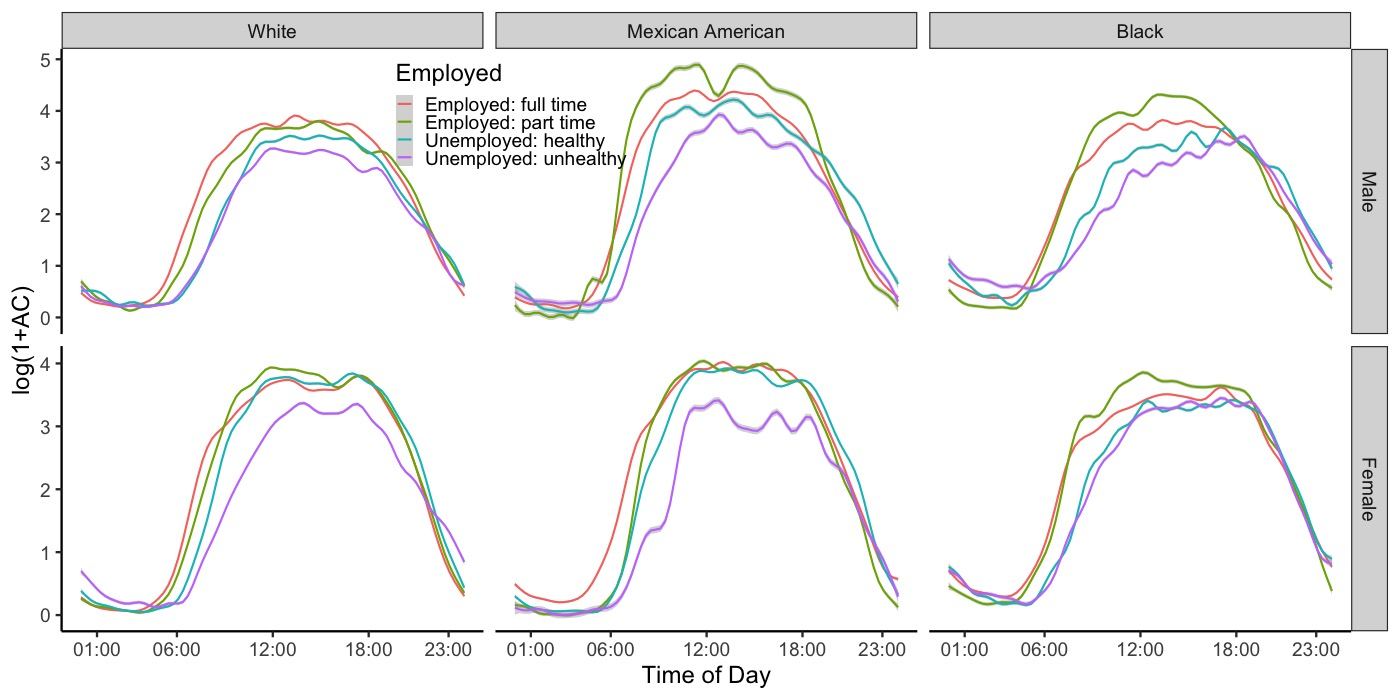
\includegraphics[width=\textwidth]{PA_profiles_by_race_employment_age_30_55_smooth}
\end{frame}





\begin{frame}
\frametitle{Physical Activity and Aging}
\begin{itemize}
\item Scientific question: How do patterns of low/light activity change with age? Do these patterns differ between weekends and weekdays? By gender? \pause
\item $i = 1,\ldots,N$ subject, $j = 1,\ldots, J_i$ day, $t = 1,\ldots,1440$ minute of the day
\item Let $M_i$ be the indicator that subject $i$ is male, and $D_{ij}$ be the indicator that day $j$ for subject $i$ is a weekend
\scriptsize
\begin{align*}
\log(1+\text{AC}_{ij}(t)) &= f_0(t) + f_1(t, \text{Age}_i)M_iD_{ij} + f_2(t,\text{Age}_i)M_i(1-D_{ij}) + \\
& \hspace{1cm}  f_3(t, \text{Age}_i)(1-M_i)D_{ij} + f_4(t,\text{Age}_i)(1-M_i)(1-D_{ij})+ \epsilon_{ij}(t) \\ 
&  \hspace{0.5cm} \epsilon_i(t) \sim N(0,\sigma^2)
\end{align*} 
\normalsize
\item PA modelled as smooth function of age and time of day separately for each gender and weekday vs weekend
\item Ignores within subject correlation
\end{itemize}
\end{frame}


\begin{frame}
\frametitle{Physical Activity and aging}
\centering
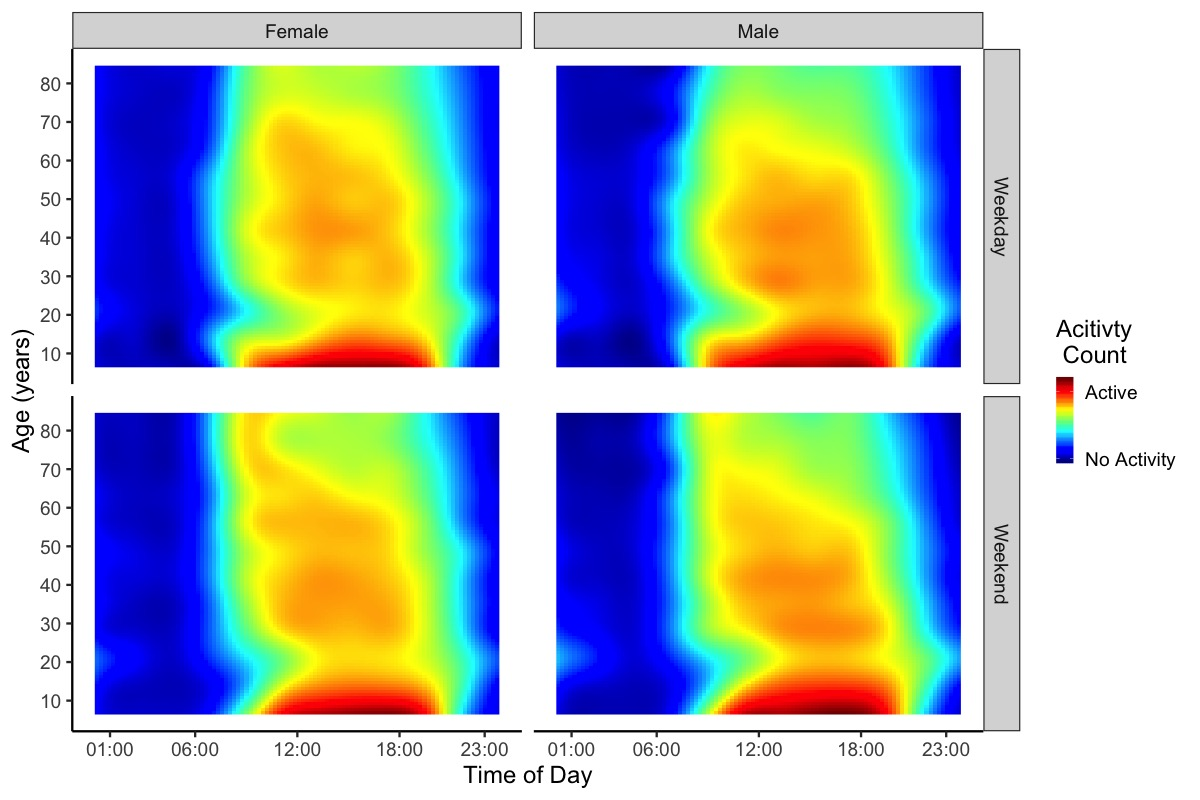
\includegraphics[width=\textwidth]{PA_profiles_by_age_by_wknd}
\end{frame}






\begin{frame}
\frametitle{Functional regression in {\it R}}
\begin{itemize}
\item In {\it R}, the main software package designed specifically for fitting functional regression models is the {\it refund} package\footnotemark
\item Basically, {\it refund} contains wrapper functions for the {\it gam()/bam()} functions in the {\it mgcv} package\footnotemark\footnotemark
\item Reduces user burden: data transformations, numeric integration, extracting estimated functional coefficients, and dealing with identifiability constraints.
\end{itemize}


\footnotetext{Goldsmith J, Scheipl F, Huang L, et al. (2018).
  refund: Regression with Functional Data. R package version 0.1-17.
  \url{https://CRAN.R-project.org/package=refund}}
\footnotetext{Wood, SN (2017). Generalized Additive Models: An Introduction with R (2nd edition). Chapman
  and Hall/CRC.}
\footnotetext{Wood, SN (2018). mgcv: Mixed GAM Computation Vehicle with GCV/AIC/REML smoothness estimation and GAMMs by REML/PQL. 
  R package version 1.8-25. \url{https://CRAN.R-project.org/package=mgcv}}

\end{frame}

% 



\section{Class Project}

\begin{frame}
\frametitle{Class Project Ideas}
\small
\begin{itemize}
\item Missing data
    \begin{itemize}
    \item (Medium/Easy) Look in depth at missing data patterns (within a day, across days, by age, etc.)
    \item (Hard) Impute missing activity data at the minute level
    \end{itemize}
\item Functional Regression [I have ideas for each of these]
    \begin{itemize}
    \item (Hard) Propose and estimate a functional transition model
    \item (Hard/Medium) Model time dependent fragmentation 
    \item (Hard/Medium) Model PA profiles using models for zero inflated count data
    \end{itemize}
\item (Medium) Try to beat TAC as a predictor of 5-year mortality
\item (Medium) Develop a Shiny application for impressive visualization of the data
\item (Medium) Assess the weekend vs. weekday effect of PA on an outcome
\item (Medium/Easy) Associate ``adjusted'' fPCA scores with mortality (patterns unaccounted for by age-, sex- specfic average activity) 
\end{itemize}
\end{frame}






\end{document}
